\chapter{ECUACIONES DE CONSERVACIÓN Y SISTEMAS HIPERBÓLICOS DE PRIMER ORDEN}
En este capítulo se introducen los conceptos fundamentales de las ecuaciones de conservación y sistemas hiperbólicos de primer orden. También se introduce el problema de Riemann asociado a una ecuación de conservación. Los desarrollos de los conceptos en este capítulo están basados en la presentación del tema realizada por Randall LeVeque \cite{LeVeque}, especialmente en los capítulos \textit{The Derivations of Conservation Laws}, \textit{Scalar Conservations Laws}, \textit{Scalar Examples} y \textit{Linear Hyperbolic Systems}.
\section{Ecuaciones de conservación}
\label{sec:ecuaciones-de-conservacion}
En física, una ecuación de conservación es una ecuación diferencial parcial de la siguiente forma
\begin{equation}
	\pdv{\mathbf{U}}{t} + \pdv{\mathbf{F}(\mathbf{U})}{x} = 0
	\label{eq:conservacion}
\end{equation}
o utilizando una notación más compacta para las derivadas,
\begin{equation}
	\mathbf{U}_{t} + \mathbf{F}(\mathbf{U})_{x} = 0
	\label{eq:conserv-deriv-short}
\end{equation}
donde $\mathbf{U}$ es un vector n-dimensional de variables físicas que se conservan, por ejemplo, la densidad, la masa o el momentum de un medio. En este texto, las variables de las que depende $\mathbf{U}$ dependen de $x$ y $t$, una variable espacial y otra temporal respectivamente. Por tanto, $\mathbf{U}$ se define formalmente como $\mathbf{U} : \mathbb{R} \times  \mathbb{R} \rightarrow \mathbb{R}^{n}$, mientras que la i-ésima variable conservada se denomina $\mathbf{u}_{i}$, de tal manera que $\mathbf{U} = \mathbf{U}(\mathbf{u}_{1}, \mathbf{u}_{2}, \dots, \mathbf{u}_{n})$. 

La función $\mathbf{F}$ corresponde al \textbf{flujo} de cada una de las variables involucradas en un punto $(x,t)$. Al igual que $\mathbf{U}$, la función $\mathbf{F}$ depende de las mismas variables físicas y por ende, también depende de $(x,t)$. Sin embargo, el flujo de cada variable conservada puede tener una forma distinta, entonces es conveniente escribir a $\mathbf{F}$ como un vector de $n$ funciones independientes, $\mathbf{F} = (\mathbf{f}_{1}, \mathbf{f}_{2}, \dots, \mathbf{f}_{n})$
de tal manera que $f_i$ es la función de flujo de la i-ésima variable conservada, $u_i$.

Una ecuación de conservación para un sistema definido en un intervalo espacial $D = [a,b]$ necesita de condiciones iniciales para su resolución, el caso más simple a considerar es el de un problema de Cauchy. En dicho caso, se debe especificar una función $\mathbf{U}_0(x)$
\begin{equation}
	\mathbf{U}(x,0) = \mathbf{U}_0(x)
\end{equation} 
la cual sea válida para todo $x$ tal que $x \in D$ y condiciones de frontera
\begin{equation}
	\mathbf{U}(a,t) = \mathbf{U}_{a}
\end{equation}
\begin{equation}
	\mathbf{U}(b,t) = \mathbf{U}_{b}
\end{equation}
con $\mathbf{U}_{a}$ y $\mathbf{U}_{b}$ fijos.

Otra forma de escribir una ecuación de conservación es utilizando la matriz jacobiana $\mathbf{A(\mathbf{U})}$ definida como
\begin{equation}
	\mathbf{A(\mathbf{U})} \equiv
	\begin{bmatrix}
		\pdv{\mathbf{f}_1}{u_1} & \dots & \pdv{\mathbf{f}_1}{u_n} \\
		\vdots & \ddots & \vdots \\
		\pdv{\mathbf{f}_n}{u_1} & \dots & \pdv{\mathbf{f}_n}{u_n} \\
	\end{bmatrix}
\end{equation}
de tal manera que la ecuación (\ref{eq:conservacion}) se convierte en
\begin{equation}
	\mathbf{U}_{t} + \mathbf{A(\mathbf{U})}\mathbf{U}_{x} = 0
	\label{eq:conservacion-jacobiana}
\end{equation}.
Esta forma de escribir una ecuación de conservación es relevante ya que permite definir un \textbf{sistema hiperbólico}. Un sistema hiperbólico es una ecuación de conservación de la forma (\ref{eq:conservacion-jacobiana}) tal que los autovalores de la matriz $\mathbf{A(\mathbf{U})}$ para todo $\mathbf{U}$ sean reales y que dicha matriz sea diagonalizable. Esto implica que existen $n$ vectores propios linealmente independientes de $\mathbf{A(\mathbf{U})}$.
Una ecuación de conservación depende de una función $\mathbf{F(\mathbf{U})}$ que, por lo general, no es una función lineal de $\mathbf{U}$, lo que implica que las ecuaciones de conservación son regularmente no lineales. Esto también se puede inferir por la dependencia en $\mathbf{U}$ de la matriz $\mathbf{A}$ en la ecuación (\ref{eq:conservacion-jacobiana}).
\section{Derivación de una ecuación de conservación}
El principio físico de una ecuación de conservación es más explícito cuando esta se deriva a través de cantidades expresadas en forma \textbf{integral.} Considerando un ejemplo de la mecánica de fluidos, se define $M(x_1,x_2,t)$ como la cantidad de masa de un fluido que se encuentra contenido en un ``tubo'' unidimensional en un intervalo  $[x_1,x_2]$ en un tiempo $t$. Si a dicho fluido se le asocia una densidad $\rho(x,t)$, entonces esta última se define de tal manera que su integral definida en un intervalo espacial sea igual a la masa contenida en ese mismo intervalo, i.e.,
\begin{equation}
	M(x_1, x_2, t) = \int_{x_1}^{x_2}\rho(x,t)\dd{x}.
\end{equation}
Ahora, asumiendo que el tubo es cerrado e impenetrable, la cantidad de masa en una región arbitraria $[x_1,x_2]$ puede variar solamente a causa de que el fluido se desplace (fluya) a través de los puntos límites de la región, $x_1$ y $x_2$. Para cuantificar el flujo que sale o entra en una región se necesita la velocidad del fluido, $v(x,t)$. Cabe destacar que debido a que el fluido se mueve en un espacio unidimensional, su velocidad se limita a dirigirse en el mismo sentido espacial, es decir, su velocidad tiene dirección sobre $x$. Entonces el flujo del fluido en un punto $(x,t)$, $F(x,t)$, se define como 
\begin{equation}
	F(x,t) = \rho(x,t)v(x,t)
\end{equation}.
Entonces, como previamente se comentó, se puede escribir la razón instantánea de cambio de masa en la región $[x_1,x_2]$ en términos del flujo entrante y saliente de la misma región
\begin{equation}
	\dv{t}	\left[M(x_1, x_2, t)\right] = F(x_2,t) - F(x_1,t)
\end{equation}
\begin{equation}
	\dv{t}	\int_{x_1}^{x_2}\rho(x,t)\dd{x} = \rho(x_2,t)v(x_2,t) - \rho(x_1,t)v(x_1,t)
	\label{eq:continuidad-1-integral}
\end{equation}
Esta es la forma integral de una ecuación de conservación. En particular, esta ecuación refleja el principio de conservación de la masa y a su vez es conocida como \textbf{ecuación de continuidad}. La ecuación (\ref{eq:continuidad-1-integral}) se puede integrar en el tiempo para conseguir expresarla independientemente de cualquier derivada, obteniendo
\begin{equation}
	\int_{t_1}^{t_2}\dv{t}\int_{x_1}^{x_2}\rho(x,t)\dd{x}\dd{t}  = \int_{t_1}^{t_2}\left[\rho(x_2,t)v(x_2,t) - \rho(x_1,t)v(x_1,t)\right]\dd{t}
\end{equation}
\begin{equation}
	\int_{x_1}^{x_2}[\rho(x,t_2) - \rho(x,t_1)]\dd{x}  = \int_{t_1}^{t_2}\left[\rho(x_2,t)v(x_2,t) - \rho(x_1,t)v(x_1,t)\right]\dd{t} 
	\label{eq:continuidad-2-integral}.
\end{equation}
Asumiendo que $t_1<t_2$, esta igualdad ofrece una expresión para la diferencia de masa contenida en la región $[x_1,x_2]$ entre los instantes $t_2$ y $t_1$. 

Es posible obtener una forma diferencial partiendo de la forma integral de una ecuación de conservación, pero es necesario asumir que las funciones $\rho(x,t)$ y $v(x,t)$ son \textbf{diferenciables}. Esta última característica que se exige en las funciones entra en conflicto cuando se estudian soluciones\footnote{Dichas soluciones se conocen como \textbf{soluciones débiles}, tema que se abordará a detalle más adelante.} de las ecuaciones de conservación con discontinuidades. Por lo tanto, la forma integral de las ecuaciones es utilizada al estudiar problemas con dichas características. Para convertir la ecuación en forma integral a su forma diferencial, se tienen que usar las siguientes expresiones:
\begin{equation}
	\rho(x,t_2)-\rho(x,t_1) = \int_{t_1}^{t_2}\pdv{t}\rho(x,t)\dd{t}
\end{equation}
y
\begin{equation}
	\rho(x_2,t)v(x_2,t)-\rho(x_1,t_1)v(x_1,t) = \int_{x_1}^{x_2}\pdv{x}\rho(x,t)v(x,t)\dd{x}
\end{equation}
sustituyendo estas expresiones en (\ref{eq:continuidad-2-integral}) se obtiene
\begin{equation}
	\int_{t_1}^{t_2}\int_{x_1}^{x_2}\left[\pdv{\rho(x,t)}{t} + \pdv{\rho(x,t)v(x,t)}{x}\right]\dd{x}\dd{t} = 0.
	\label{eq:integral-con-derivadas}
\end{equation}
Puesto que la ecuación (\ref{eq:integral-con-derivadas}) se cumple para cualquier punto $(x,t)$ del dominio, el integrando de la misma debe ser idénticamente cero. Entonces,
\begin{equation}
	\rho_{t} + (\rho v)_{x} = 0
\end{equation}
es la forma diferencial de la ecuación de conservación de la masa, así como se definió una ecuación de conservación en (\ref{eq:conserv-deriv-short}), ya que la función de flujo se definió como $F = \rho v$. Puesto que la ecuación diferencial de conservación de la masa involucra dos cantidades físicas, esta se puede resolver ya sea si se conoce previamente la función $v(x,t)$ o si esta última se puede escribir como una función de $\rho$, i.e., $v=v(\rho)$. En este último caso la ecuación de conservación de la masa es una ecuación diferencial parcial únicamente para $\rho$ y toma la siguiente forma
\begin{equation}
	\rho_t + f(\rho)_x = 0.
\end{equation}
Esta última es un ejemplo de \textbf{ecuación de conservación escalar} ya que solamente interviene una incógnita, $\rho$.
En caso que la velocidad $v(x,t)$ sea una constante $\alpha$, la ecuación de conservación de la masa se convierte en:
\begin{equation}
	\rho_t + \alpha\rho_x = 0,
	\label{eq:adveccion}
\end{equation}
esta ecuación se conoce como \textbf{ecuación de advección lineal} o como ecuación de onda de primer orden \cite{heattransfer}.
\section{Ecuación de advección lineal}
La ecuación de advección (\ref{eq:adveccion}) con la siguiente condición inicial:
\begin{equation}
	\rho(x,0) = \rho_0(x), \hspace{1.7cm} -\infty < x < \infty,
\end{equation}
tiene como solución:
\begin{equation}
	\rho(x,t) = \rho_0(x - \alpha t),
	\label{eq:sol-advec}
\end{equation}
para $t> 0$, asumiendo que $\rho_0$ es una función diferenciable. Esta solución se puede interpretar como la traslación de la función $\rho_0$ a lo largo del eje $x$ con una velocidad $\alpha$, en la misma dirección de la velocidad, es decir, a la derecha si $\alpha > 0$ y a la izquierda si $\alpha < 0$.
\subsection{Curvas características}
Se puede demostrar que la solución (\ref{eq:sol-advec}) es constante respecto al tiempo a lo largo de cada curva definida por $x-\alpha t = x_0$, para cualquier $x_0$ tal que $x_0 \in [-\infty, \infty]$. Dichas curvas de la forma $x=x(t)$ son conocidas como \textbf{curvas características} de la ecuación diferencial en cuestión. Las curvas características definen dominios en donde la ecuación diferencial parcial se puede escribir como una ecuación diferencial ordinaria. Dichas curvas se definen a partir de ecuaciones diferenciales ordinarias. En el caso de la ecuación de advección lineal (\ref{eq:sol-advec}), las características satisfacen la siguiente ecuación diferencial:
\begin{equation}
	\dv{x}{t} = \alpha, \hspace{1.7cm} x(0) = x_0,
\end{equation}
cuya solución es: $x-\alpha t = x_0$. Para demostrar que la ecuación de advección lineal se convierte en una ecuación diferencial ordinaria a lo largo de dichas curvas, se deriva la función incógnita $\rho$ respecto al tiempo,
\begin{equation}
	\dv{\rho}{t} = \pdv{\rho}{t} + \pdv{\rho}{x}\dv{x}{t}
\end{equation}
\begin{equation}
	\dv{\rho}{t} = \pdv{\rho}{t} + \alpha\pdv{\rho}{x}
\end{equation}
\begin{equation}
	\dv{\rho}{t} = 0,
\end{equation}
este último paso toma efecto dado que a lo largo de las curvas características, $\dv{x}{t} = \alpha$. Se puede notar que en este último procedimiento se recuperó la ecuación diferencial en cuestión (\ref{eq:sol-advec}), expresada como una ecuación diferencial ordinaria y concluyó al igualar la derivada temporal a cero, consiguiendo demostrar que $\rho$ es constante a lo largo de las características.
\section{Dominio de dependencia de una ecuación de conservación}
En la sección anterior se introdujo el concepto de curvas características de una ecuación de conservación y en el caso de la ecuación de advección, es posible obtener la solución general utilizando la expresión para sus características, esto es $x(t) = x_0 + \alpha t$. Por lo tanto, se puede afirmar que el valor de $\rho(x,t)$ para un instante $(x',t')$ depende de la condición inicial $\rho_0$ únicamente en un solo punto $x'_{0}$ ya que $\rho$ es constante a lo largo de la curva característica $x' = x^{'}_{0} + \alpha t$. Entonces, sin importar de qué manera se cambien los valores que toma $\rho_0(x)$, mientras no se cambie su valor en $x'_0$, el valor $\rho(x',t')$ permanecerá sin cambiar. 

En el caso general, para cualquier sistema hiperbólico, el valor de la solución $\mathbf{U}$ en un punto $(x',t')$ depende únicamente de los valores que toma la función inicial $\mathbf{U}_0$ en un dominio $D(x',t')$ que corresponde a un intervalo \textbf{cerrado}. Este último se denomina \textbf{dominio de dependencia}. El tamaño de este intervalo usualmente crece a medida que avance el tiempo, sin embargo, el tamaño está acotado de la siguiente forma $D(x',t') = \{x : |x-x'| \leq a_{\text{máx}}t \}$. En resumen, las ecuaciones hiperbólicas poseen una velocidad finita de propagación; lo que significa que la información de la solución puede viajar a lo largo del espacio a una velocidad $a_{\text{máx}}$ como máximo.

\section{Discontinuidades en soluciones}
Al derivar la forma diferencial de una ecuación de conservación (\ref{eq:integral-con-derivadas}) se enfatizó que era necesario exigir la diferenciabilidad de las cantidades conservadas. Sin embargo, si se toman en cuenta los atributos de la solución, proporcionados por las curvas características, de la ecuación de advección, resulta que el valor de la variable involucrada $\rho(x,t)$ depende únicamente del valor de la condición inicial en un punto $x_0$ tal que $x = x_0 + \alpha t$. Por esta última razón se puede concluir que, al menos para la ecuación de advección, es posible definir una solución sin exigirle que sea una función  suave. La definición de una solución con singularidades surge gracias a que la forma integral de una ecuación de conservación sí se satisface con funciones no diferenciables, a diferencia de la forma diferencial. También es importante hacer énfasis en que la forma integral de una ecuación de conservación tiene un significado físico más fundamental.

Si la condición inicial de una ecuación de conservación escalar $u_0(x)$ tiene una singularidad (discontinuidad en sí misma o en alguna derivada), en un punto $x_0$, entonces la solución de la ecuación, $u(x,t)$, también poseerá una singularidad del mismo orden en todos los puntos definidos por la característica que parte de $x_0$. Para los sistemas hiperbólicos en general, las singularidades se propagan a lo largo de las curvas características.

A continuación se describen dos formas de definir las soluciones con singularidades:
\subsection{Viscosidad disipada}
Como se vio anteriormente algunas soluciones de las ecuaciones de conservación pueden poseer singularidades si la condición inicial de la ecuación tiene una singularidad. Para los sistemas hiperbólicos no lineales, las discontinuidades pueden formarse a lo largo de la evolución temporal de la solución. A las singularidades que se desarrollan en las soluciones se les llama \textbf{ondas de choque} o \textbf{shocks} en inglés \cite{Cameron}. Para definir cómo estas funciones siguen siendo soluciones, en el sentido estricto de la palabra, se redefine la ecuación que deben satisfacer agregándole un coeficiente de viscosidad $\varepsilon$ que va acompañado del laplaciano de la variable involucrada. En el caso de la ecuación de advección para $u$, se define la siguiente ecuación modificada
\begin{equation}
	u_t + \alpha u_x = \varepsilon u_{xx},
	\label{eq:advec-difus}
\end{equation}
donde $u_{xx} \equiv \pdv[2]{u}{x}$. A esta ecuación se le conoce como \textbf{ecuación de advección - difusión}, ya que el término viscoso también se denomina como término difusivo y está involucrado en la ecuación de difusión, también conocida como ecuación de calor \cite{heattransfer}. 

Si se denota a $u^{\varepsilon}(x,t)$ como la solución de la ecuación (\ref{eq:advec-difus}) con condición inicial $u_0(x)$, entonces $u^{\varepsilon} \in C^{\infty}(\mathbb{R} \times [0,\infty)) $ donde $ C^{\infty}(\mathbb{R}\times [0,\infty))$ es el conjunto de funciones infinitamente diferenciables (suaves) definidas en el mismo espacio en donde se resuelve la ecuación. Esto se cumple incluso si $u_0(x)$ no es una función suave, ya que la ecuación (\ref{eq:advec-difus}) es de tipo parabólica. Para encontrar la solución a la ecuación original (\ref{eq:adveccion}) se debe hacer el límite $\varepsilon \rightarrow 0$ en la solución de la ecuación de advección - difusión (\ref{eq:advec-difus}); a esta forma de definir una solución con discontinuidades se le denomina \textbf{solución con viscosidad disipada}.
\subsection{Solución débil}
La otra forma de definir una solución con singularidades es definiendo una \textbf{solución débil} de la ecuación de conservación, haciendo uso de la forma integral de esta última. Es evidente que la forma diferencial de la ecuación de conservación no se satisface con una función con singularidades ya que sus derivadas no están bien definidas en todo el dominio de la función. La idea del procedimiento de la definición de una solución débil es reescribir la ecuación en forma integral, trasladando las derivadas hacia una \textbf{función prueba}, que sí es una función diferenciable y así relajar las condiciones de suavidad para la función incógnita.

Sea $\phi(x,t)$ una función continuamente diferenciable con \textbf{soporte compacto}, i.e., $\phi(x,t) \in C_{0}^{1} (\mathbb{R} \times [0, \infty))$. La tenencia de soporte compacto de la función significa que $\phi(x,t)$ es exactamente igual a cero fuera de algún conjunto cerrado, por lo que el soporte de la función yace en un subconjunto compacto del espacio $(x,t) = \mathbb{R} \times [0, \infty)$ \cite{Cameron}.

Para definir la solución débil de la ecuación de conservación escalar $u_t + f(u)_x = 0$, esta se multiplica por la función $\phi$ descrita anteriormente:
\begin{equation}
	u_t + f(u)_x = 0
	\label{eq:conser-u}
\end{equation}
\begin{equation}
	\phi u_t + \phi f(u)_x = 0.
\end{equation}
Ahora, se integra sobre todo el espacio y el tiempo,
\begin{equation}
	\int_{0}^{\infty}\int_{-\infty}^{\infty}\left(\phi u_t + \phi f(u)_x\right) \dd{x}\dd{t} = 0,
\end{equation}
luego, integrando por partes cada término de la integral, se obtiene
\begin{equation}
	\int_{-\infty}^{\infty}\int_{0}^{\infty} \phi u_t \dd{t}\dd{x} = \int_{-\infty}^{\infty}\int_{0}^{\infty} \left((\phi u)_t - \phi_t u\right) \dd{t}\dd{x}
\end{equation}
\begin{equation}
	\int_{-\infty}^{\infty}\int_{0}^{\infty} \phi u_t \dd{t}\dd{x} = \int_{-\infty}^{\infty} (\phi u) \Big|_{0}^{\infty}\dd{x} - \int_{-\infty}^{\infty}\int_{0}^{\infty}\phi_t u \dd{t}\dd{x}.
\end{equation}
Dado que $\phi$ tiene soporte compacto, es posible asegurarse que $\lim\limits_{t\rightarrow \infty}\phi(x,t) = 0$. Por tanto,
\begin{equation}
	\int_{-\infty}^{\infty}\int_{0}^{\infty} \phi u_t \dd{t}\dd{x} = 
	-\int_{-\infty}^{\infty} \phi(x,0)u(x,0) \dd{x} - \int_{-\infty}^{\infty}\int_{0}^{\infty}\phi_t u \dd{t}\dd{x}.
\end{equation}
Trabajando el segundo término, se tiene
\begin{equation}
	\int_{0}^{\infty}\int_{-\infty}^{\infty}  \phi f(u)_x \dd{x}\dd{t} = 
	\int_{0}^{\infty}\int_{-\infty}^{\infty} \left((\phi f(u))_x - \phi_x f(u)\right) \dd{x}\dd{t}
\end{equation}
\begin{equation}
	\int_{0}^{\infty}\int_{-\infty}^{\infty}  \phi f(u)_x \dd{x}\dd{t} = 
	\int_{0}^{\infty} \phi f(u) \Big|_{-\infty}^{\infty} \dd{t}  - \int_{0}^{\infty}\int_{-\infty}^{\infty} \phi_x f(u) \dd{x}\dd{t},
\end{equation}
de igual manera que con la valuación de la integral del término anterior, el soporte compacto de $\phi$ permite justificar que $\lim\limits_{x\rightarrow -\infty}\phi = 0 = \lim\limits_{x\rightarrow \infty}\phi$. Entonces,
\begin{equation}
	\int_{0}^{\infty}\int_{-\infty}^{\infty}  \phi f(u)_x \dd{x}\dd{t} =  -\int_{0}^{\infty}\int_{-\infty}^{\infty} \phi_x f(u) \dd{x}\dd{t}.
\end{equation}
Por tanto, la integral de la ecuación de conservación multiplicada por la función prueba queda como
\begin{equation}
\begin{aligned}
	\int_{0}^{\infty}\int_{-\infty}^{\infty}\left(\phi u_t + \phi f(u)_x\right) \dd{x}\dd{t} = \int_{-\infty}^{\infty} \phi(x,0)u(x,0) \dd{x} \\
	-\int_{0}^{\infty}\int_{-\infty}^{\infty}\left(\phi_t u + \phi_x f(u)\right) \dd{x}\dd{t} = 0.
\end{aligned}
\end{equation}
Por tanto, se obtiene la igualdad
\begin{equation}
	\int_{0}^{\infty}\int_{-\infty}^{\infty}\left(\phi_t u + \phi_x f(u)\right) \dd{x}\dd{t} = -\int_{-\infty}^{\infty} \phi(x,0)u(x,0) \dd{x},
	\label{eq:weak-equality}
\end{equation}
que tal y como se dijo previamente, las derivadas parciales ahora están siendo aplicadas a $\phi$ y la integral de la nueva ecuación diferencial se iguala a una integral que depende únicamente de las condiciones iniciales del problema a resolver para $u$. Entonces se dice que $u$ es una \textbf{solución débil} de la ecuación (\ref{eq:conser-u}) si y solo si se cumple la igualdad (\ref{eq:weak-equality}) para todo $\phi$ tal que $\phi(x,t) \in C_{0}^{1} (\mathbb{R} \times [0, \infty))$.

Es posible demostrar que la igualdad (\ref{eq:weak-equality}) es equivalente a la forma integral de la ecuación diferencial en cuestión (ecuación \ref{eq:continuidad-2-integral}), mediante la elección de una función de prueba que esta cumpla con la siguiente propiedad:
\begin{equation}
	\phi(x,t) = 
	\begin{cases}
		1 & \text{para } (x,t) \in [x_1, x_2] \times [t_1, t_2]\\
		0 & \text{para } (x,t) \notin [x_1 - \epsilon, x_2 + \epsilon] \times [t_1 - \epsilon, t_2 + \epsilon].
 	\end{cases}
\end{equation}
Además $\phi$ es una función suave en la banda intermedia con ancho $\epsilon$. Entonces al calcular la integral (\ref{eq:weak-equality})  se puede notar que esta se reduce a la integral sobre la banda $\epsilon$, a raíz de la propiedad expuesta anteriormente. Al calcular esta integral y haciendo el límite $\epsilon \rightarrow 0$, las derivadas $\phi_x$ y $\phi_t$ tienden a deltas de Dirac \footnote{La delta de Dirac $\delta(x)$ es una función generalizada que cumple con la siguiente propiedad $\int_{-\infty}^{\infty} \delta(x-a) f(x)\dd{x} = f(a)$ \cite{methods}.}, recuperando así los valores de $u$ y $ f(u)$ en las fronteras del dominio $ [x_1, x_2] \times [t_1, t_2]$ en integrales que equivalen a los términos de la ecuación de conservación en forma integral (\ref{eq:continuidad-2-integral}). Cabe destacar que este es un esbozo solamente de la demostración, ya que esta requiere más rigor matemático. Sin embargo, lo imprescindible es destacar la equivalencia entre ambas expresiones.

La solución de viscosidad disipada también califica como una solución débil y físicamente es la solución correcta. Existen muchas soluciones débiles, incluyendo algunas que no tienen un significado físico consistente, para ello es necesario exigir otras condiciones sobre las soluciones débiles de tal manera que se obtenga la solución correcta. Estas condiciones son conocidas como \texttt{condiciones de entropía} por su papel en la dinámica de fluidos.

\section{Ecuación de Burgers}
Se pueden destacar las propiedades más importantes de las ecuaciones de conservación no lineales de la mecánica de fluidos a través de un ejemplo escalar conocido como \textbf{ecuación de Burgers.} Esta ecuación tiene la siguiente forma:

\begin{equation}
	u_t + u u_x = 0,
	\label{eq:burgers}
\end{equation}
la cual es formalmente conocida como Ecuación de Burgers sin viscosidad, pero en este texto se le referirá solamente como Ecuación de Burgers. Esta ecuación es un modelo muy simple de la velocidad $u$ de un gas \cite{Cameron}. La ecuación originalmente estudiada por Jan Burgers contiene un término de viscosidad cinemática:
\begin{equation}
	u_t + u u_x = \varepsilon u_{xx},
	\label{eq:burgers-vis}
\end{equation}
donde $\varepsilon$ es el coeficiente de viscosidad cinemática. A esta última ecuación se le referirá como Ecuación de Burgers viscosa.

De la ecuación (\ref{eq:burgers}) podemos notar un ligero parecido a la ecuación de advección (\ref{eq:adveccion}), con la diferencia que la velocidad de advección $\alpha$ se reemplaza por la variable que sufre la advección, i.e., $u$, lo que brinda la naturaleza no lineal de este modelo. La ecuación de Burgers se puede escribir en forma conservativa:
\begin{equation}
	u_t + \left(\frac{1}{2}u^{2}\right)_x = 0.
	\label{eq:burgers-cons}
\end{equation}
A partir de esta forma, se puede concluir que la función de flujo es $f(u) = \frac{1}{2}u^{2}$.
\subsection{Curvas características}
Las curvas características de la ecuación de Burgers se pueden definir a través de la siguiente ecuación diferencial
\begin{equation}
	x'(t) = u(x(t),t),
	\label{eq:burgers-char}
\end{equation}
dado que se puede recuperar la ecuación diferencial parcial derivando respecto al tiempo la velocidad:
\begin{equation}
	\dv{t} u(x(t),t) = \pdv{u}{t} + \pdv{u}{x} \dv{x}{t}
\end{equation}
\begin{equation}
	\dv{t} u(x(t),t) = \pdv{u}{t} + u\pdv{u}{x} = 0.
\end{equation}
Por lo tanto, $u$ es constante en el tiempo sobre cualquier característica. Se puede resolver la ecuación (\ref{eq:burgers-char}) utilizando este último hecho:
\begin{equation}
	x(t) = u(\xi,0)t + \xi
	\label{eq:burg-char-expr}
\end{equation}
y al resolver para $\xi$, es posible resolver la ecuación diferencial
\begin{equation}
	u(x,t) = u(\xi, 0).
	\label{eq:sol-burgers-char}
\end{equation}
Es importante destacar que la expresión (\ref{eq:sol-burgers-char}) para $u(x,t)$ no es válida para todo $t$, dado que las características definidas por la ecuación (\ref{eq:burg-char-expr}) pueden intersectarse en algún momento. Esto se da si para algún $x$, se tiene que $u_0'(x) < 0$. 

\begin{figure}
	\begin{subfigure}{0.5\textwidth}
		\centering
		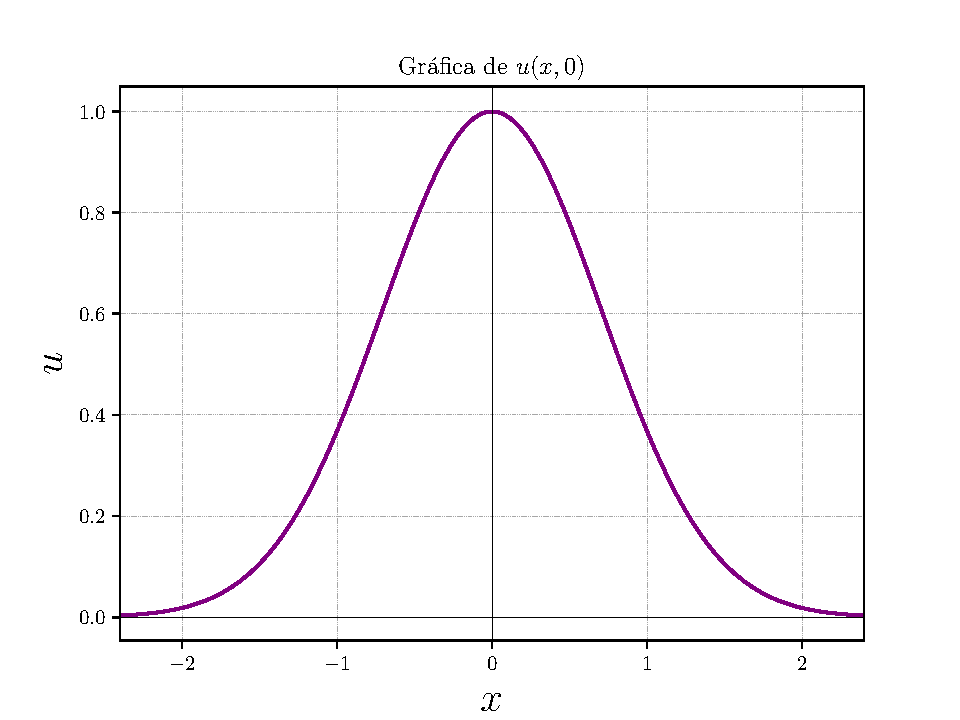
\includegraphics[width=\linewidth]{../some_plots/cond_inicial.pdf}
		\caption{Gráfica de $u(x,0) = \exp(-x^2)$.}
		\label{fig:subfig1}
	\end{subfigure}
	\begin{subfigure}{0.5\textwidth}
		\centering
		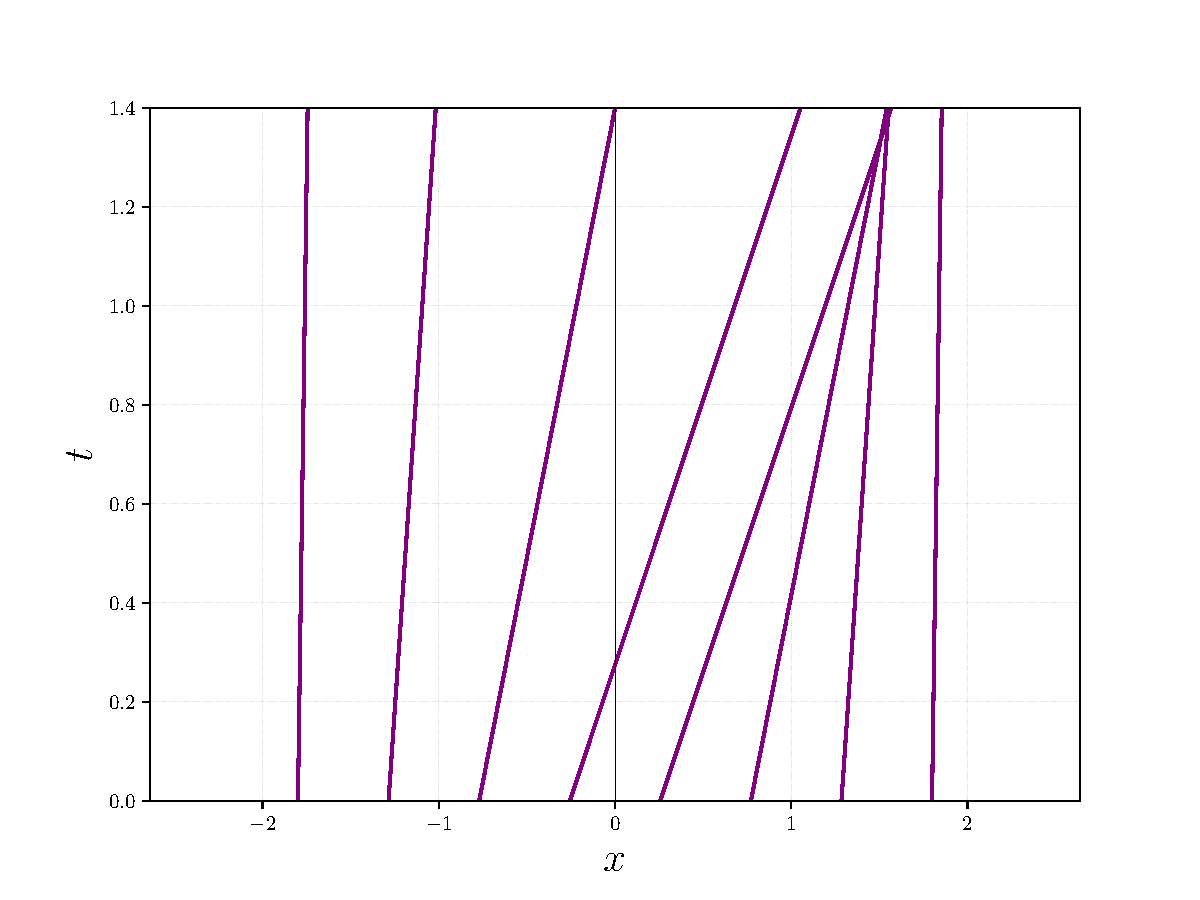
\includegraphics[width=\linewidth]{../some_plots/caracteristicas_burgers.pdf}
		\caption{Características de la ecuación de Burgers.}
		\label{fig:subfig2}
	\end{subfigure}
	\caption{Gráficas de la condición inicial $u(x,0) = \exp(-x^2)$ para la ecuación de Burgers y de algunas características asociadas a esta condición inicial. \textbf{Fuente:} elaboración propia.}
	\label{fig:figura_completa}
\end{figure}
\subsection{Ondas de choque}
Como se puede observar en la figura (\ref{fig:subfig2}), las características asociadas a una condición inicial con forma gaussiana se intersectan. Entonces, si las características se intersectan, la expresión (\ref{eq:sol-burgers-char}) no está bien definida, sino que $u(x,t)$ puede tomar varios valores a la vez, cada uno correspondiente a una característica diferente. En el caso de la ecuación de Burgers, cuando las características se intersectan, la solución se convierte en una ``función'' con tres valores distintos. Esta solución puede tener sentido en algunos contextos, como en el caso del problema de agua superficial. Sin embargo, en la mayoría de los casos esta solución no tiene significado físico. Por ejemplo, en la ecuación de Burgers la variable $u(x,t)$ representa una velocidad y esta debe devolver un solo valor.

La solución con el comportamiento físico correcto cuando las características se intersectan corresponde a una discontinuidad que se propaga con una velocidad determinada. Este efecto se puede demostrar a través del formalismo de la viscosidad disipada. Al obtener la solución de la ecuación de Burgers viscosa (\ref{eq:burgers-vis}), el parámetro $\varepsilon u_{xx}$ evita que la solución presente una discontinuidad, dado que cuando la onda comienza a presentar el choque, la segunda derivada de $u$ crece más rápido que su primera derivada. Así, al efectuar el límite de $\varepsilon \rightarrow 0$ se puede obtener una discontinuidad absoluta que corresponde a la solución de la ecuación de Burgers sin viscosidad. La tendencia de adquirir una discontinuidad  de las soluciones con menos viscosidad se puede evidenciar en la figura (\ref{fig:viscosas}).

\begin{figure}[ht]
	\begin{subfigure}{0.5\textwidth}
		\centering
		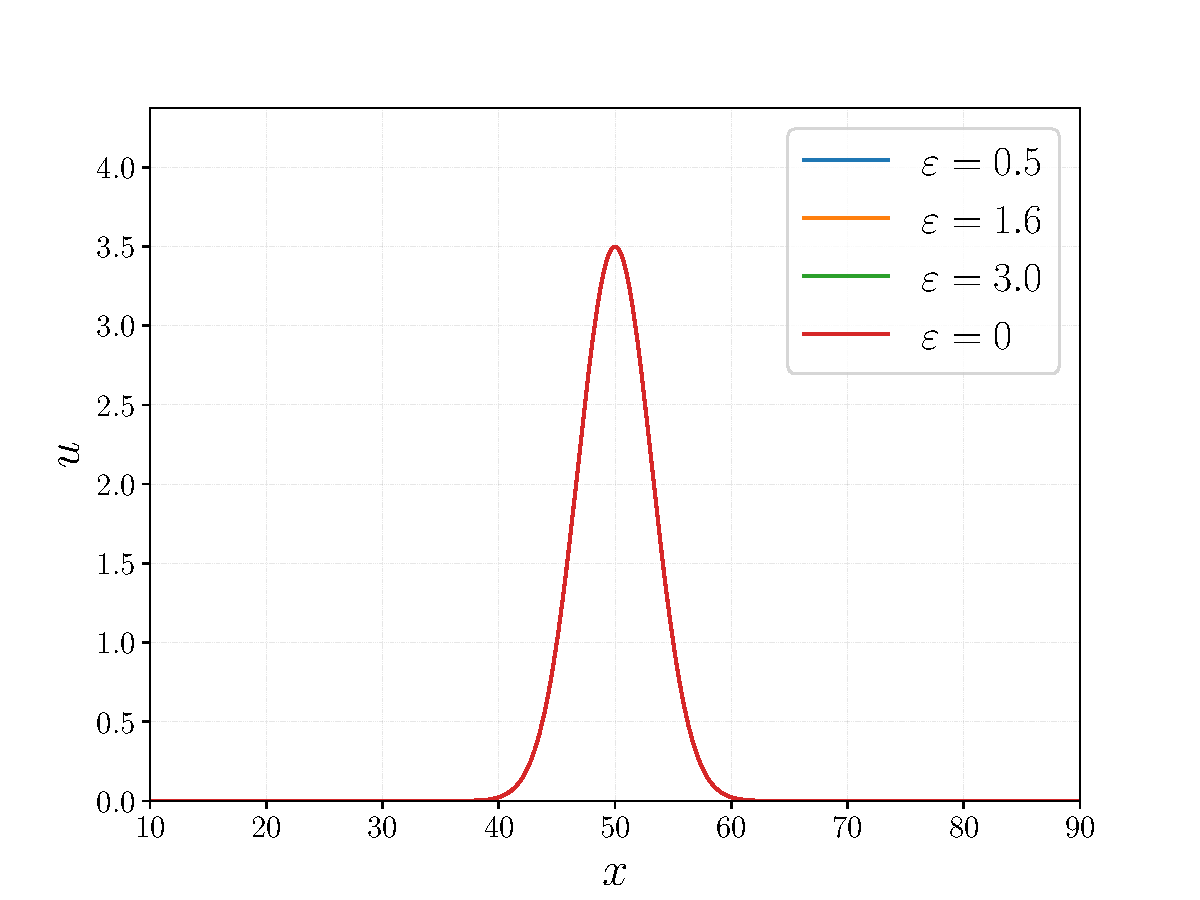
\includegraphics[width=\linewidth]{../some_plots/burgers-viscosas/graficas/viscosidades-1.pdf}
		\label{fig:viscosas1}
	\end{subfigure}
	\begin{subfigure}{0.5\textwidth}
		\centering
		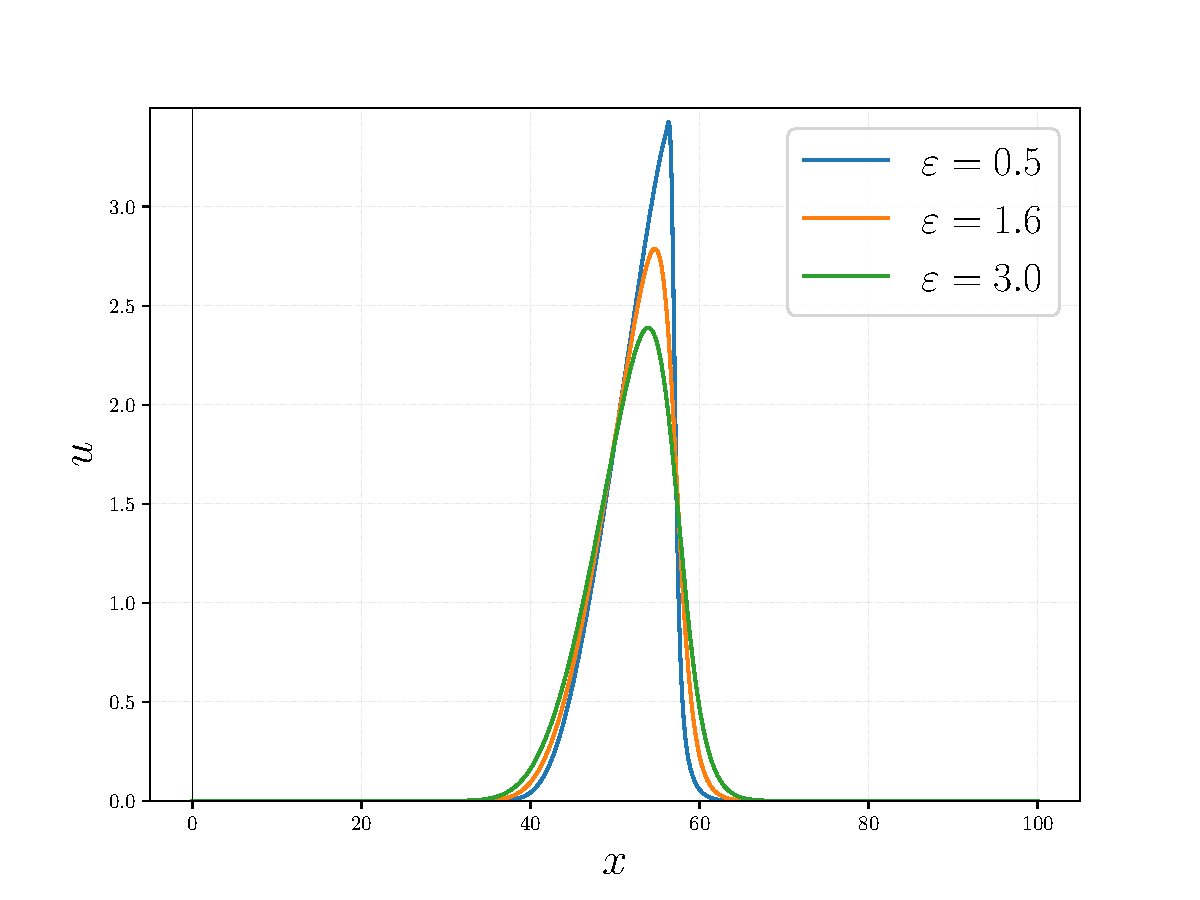
\includegraphics[width=\linewidth]{../some_plots/burgers-viscosas/graficas/viscosidades-100.pdf}
		\label{fig:viscosas2}
	\end{subfigure}
	\begin{subfigure}{0.5\textwidth}
		\centering
		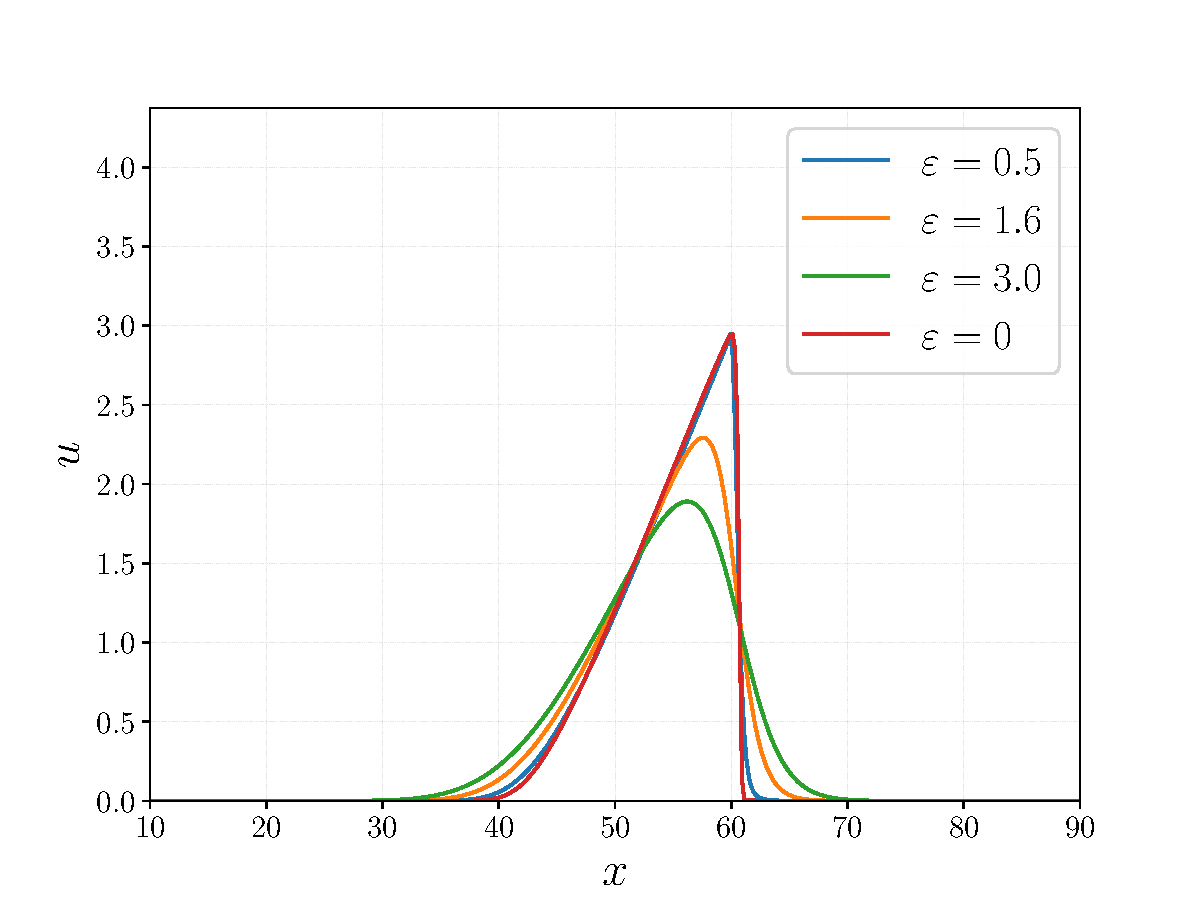
\includegraphics[width=\linewidth]{../some_plots/burgers-viscosas/graficas/viscosidades-200.pdf}
		\label{fig:viscosas3}
	\end{subfigure}
	\begin{subfigure}{0.5\textwidth}
		\centering
		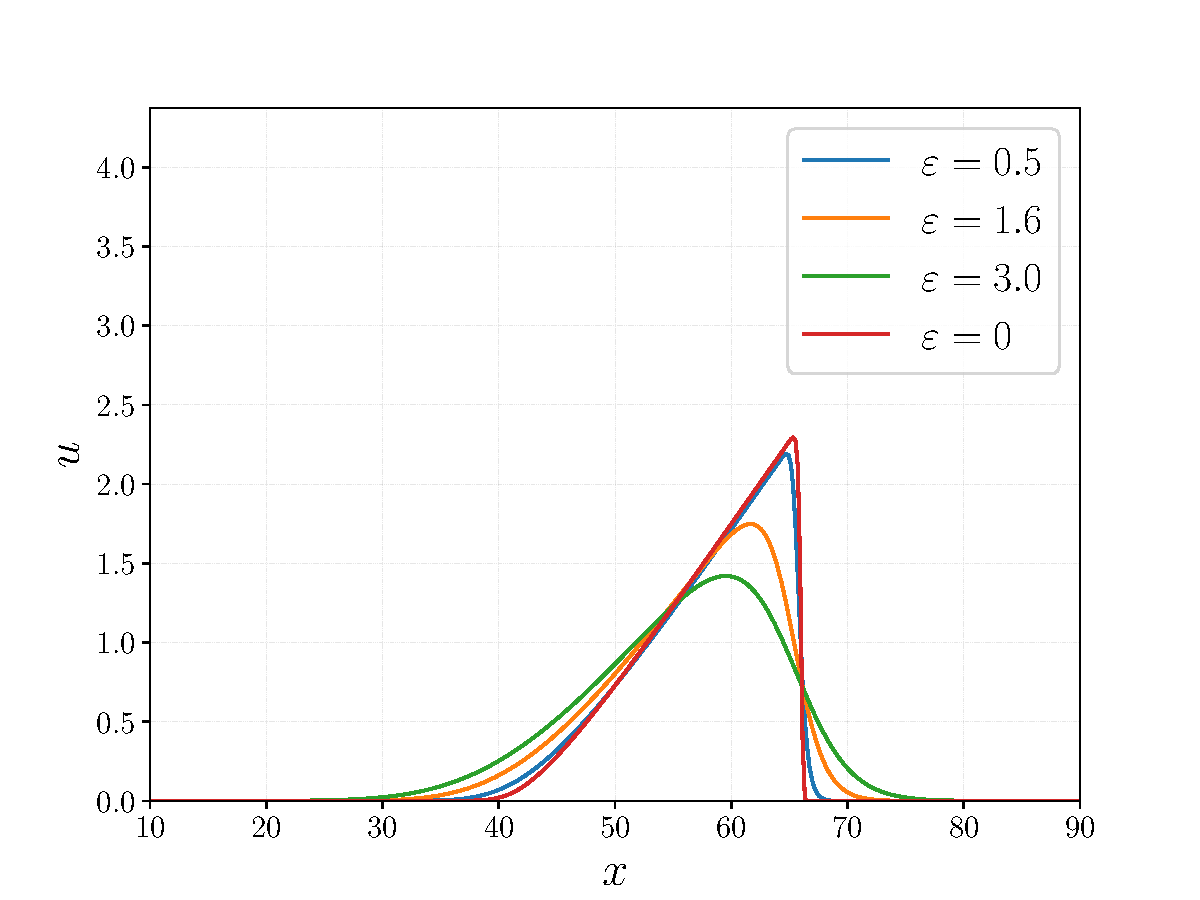
\includegraphics[width=\linewidth]{../some_plots/burgers-viscosas/graficas/viscosidades-400.pdf}
		\label{fig:viscosas4}
	\end{subfigure}
	\caption{Gráficas de las soluciones numéricas, en distintos instantes de tiempo, de la ecuación de Burgers viscosa para distintos valores de coeficiente de viscosidad cinemática ($\varepsilon$), incluyendo el caso donde no hay viscosidad (en rojo). \textbf{Fuente:} elaboración propia.}
	\label{fig:viscosas}
\end{figure}

\section{Problema de Riemann}
Como se ha mostrado, las soluciones a las ecuaciones de conservación admiten soluciones débiles que pueden presentar discontinuidades tanto en la condición inicial como en la evolución temporal de las mismas. Por esta razón, es natural estudiar ecuaciones de conservación con condiciones iniciales discontinuas. Este problema es conocido como \textbf{problema de Riemann}. En el caso escalar, el problema de Riemann para una ecuación de conservación de la forma $u_t + f(u)_x = 0$ corresponde a la siguiente condición inicial
\begin{equation}
	u(x,0) = 
	\begin{cases}
		u_L & \text{si } x < 0 \\
		u_R & \text{si } x \geq 0,
		\label{eq:riemannLR}
	\end{cases}
\end{equation}
en donde la solución es determinada por la relación entre $u_L$ y $u_R$.
\subsection{Solución al problema de Riemann para la ecuación de Burgers}
Para encontrar la solución al problema de Riemann de la ecuación de Burgers es necesario considerar dos casos.
\subsubsection{Caso $u_L > u_R$:}
La función
\begin{equation}
	u(x,t) = 
	\begin{cases}
		u_L, & \hspace{3mm} x < st \\
		u_R, & \hspace{3mm} x > st,		
	\end{cases}\label{eq:solriemannLR}
\end{equation}
conocida como \textbf{onda de choque}, representa una discontinuidad trasladándose a través del eje $x$ con una velocidad $s$. Esta última es una solución débil de la ecuación de Burgers, para la condición inicial (\ref{eq:riemannLR}), si se cumple la condición general de  \textbf{Rankine - Hugoniot} \cite{Cameron}, que se define como:
\begin{equation}
	f(u_L) - f(u_R) = s(u_L - u_R),
	\label{eq:rankinehugo}
\end{equation}
donde $f(u) = \frac{1}{2} u^{2}$. A continuación se demuestra la expresión general de la condición Rankine - Hugoniot.\\

\textit{Prueba:} Sea $u$ una solución débil de la ecuación diferencial $u_t + f(u)_x = 0$, de la forma (\ref{eq:solriemannLR}). Sea $\mathcal{M} \gg st$. Aplicando la expresión (\ref{eq:continuidad-1-integral}) a $u$:
\begin{equation}
	\dv{t} \int_{-\mathcal{M}}^{\mathcal{M}}u(x,t)\dd{x} = f(u_L) - f(u_R).
	\label{eq:flux_diff}
\end{equation}
Integrando $u$ a partir de su definición (\ref{eq:solriemannLR}), se tiene
\begin{equation}
	\int_{-\mathcal{M}}^{\mathcal{M}}u(x,t)\dd{x} = (\mathcal{M} + st)u_L + (\mathcal{M} - st)u_R.
\end{equation}
Entonces, sustituyendo en (\ref{eq:flux_diff}),
\begin{equation}
	\dv{t}\left[(\mathcal{M} + st)u_L + (\mathcal{M} - st)u_R\right] = f(u_L) - f(u_R)
\end{equation}
\begin{equation}
	s(u_L - u_R) = f(u_L) - f(u_R),
\end{equation}
se obtiene la condición de salto de Rankine - Hugoniot.

Por lo tanto, para el caso $u_L > u_R$, la solución de la ecuación de Burgers es una discontinuidad que se propaga con una velocidad constante $s = \frac{u_L + u_R}{2}$ \cite{Cameron}.

\begin{figure}[ht]
	\centering
	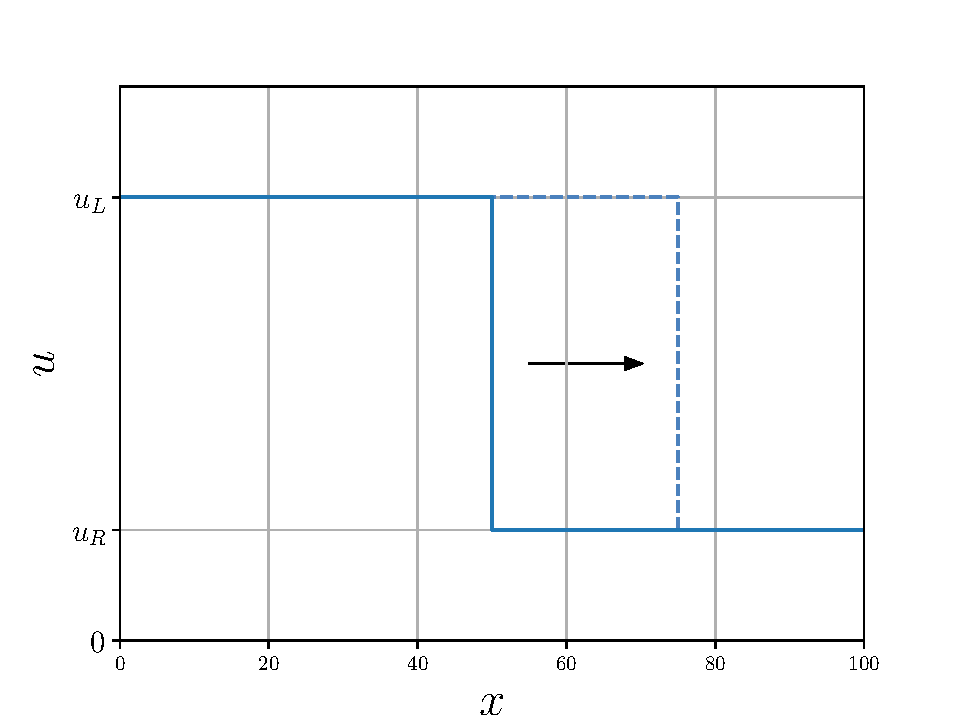
\includegraphics[width=0.8\linewidth]{../some_plots/cap1/graficas/riemannLR.pdf}
	\caption{Ejemplo gráfico de la solución de la ecuación de Burgers para el caso $u_L > u_R$. \textbf{Fuente: }elaboración propia, basada en el esquema obtenido de \cite{LeVeque}.}
	\label{fig:solriemannLR}
\end{figure}

\subsubsection{Caso $u_L < u_R$:}
Hay múltiples soluciones débiles para este caso, por ejemplo, la solución (\ref{eq:solriemannLR}) \cite{Cameron}. Sin embargo, esta no es la solución que corresponde a la solución con viscosidad disipiada \cite{Cameron}. La solución
\begin{equation}
	u(x,t) = 
	\begin{cases}
		u_L, & \hspace{3mm} x < u_{L}t \\
		x/t, & \hspace{3mm} u_{L}t \leq x \leq u_{R}t \\
		u_R, & \hspace{3mm} x > u_{R}t,		
	\end{cases}\label{eq:solriemannRL}
\end{equation}
es la solución correspondiente a la solución con viscosidad disipada y es conocida como una \textbf{onda de rarefacción}. Resulta ser poco práctico tener que recurrir frecuentemente a la solución de viscosidad disipada para encontrar la solución a cualquier caso del problema de Riemann, por lo que en su lugar se suelen imponer condiciones conocidas como \textbf{condiciones de entropía} que son equivalentes a exigir que la solución sea consistente con el formalismo de viscosidad disipada.

\begin{figure}[ht]
	\begin{subfigure}{0.5\textwidth}
		\centering
		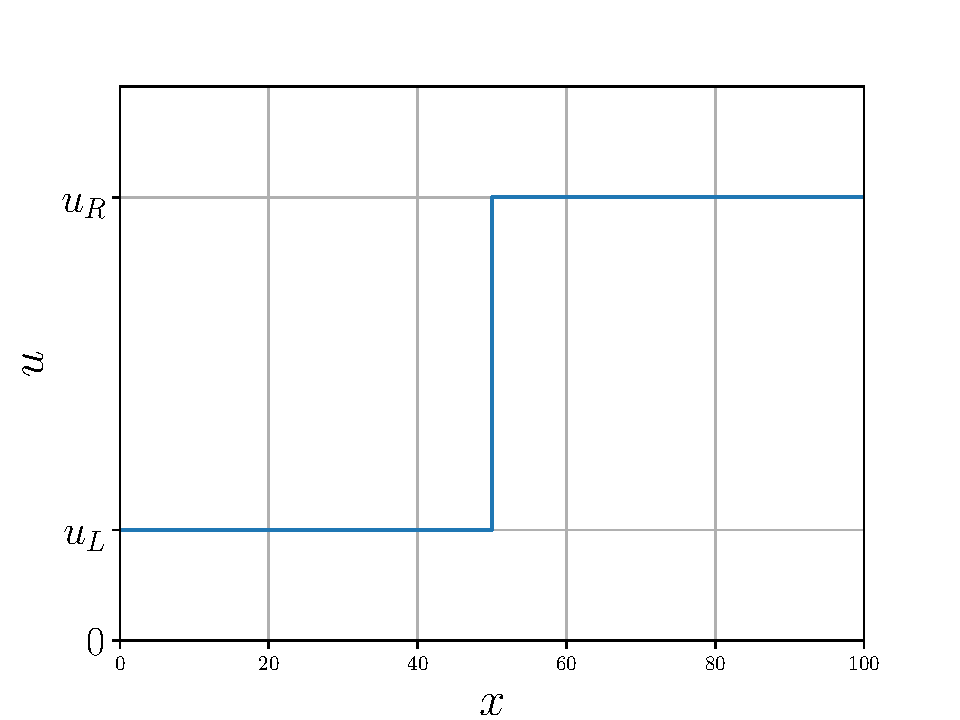
\includegraphics[width=\linewidth]{../some_plots/cap1/graficas/riemannRL-0.pdf}
	\end{subfigure}
	\begin{subfigure}{0.5\textwidth}
		\centering
		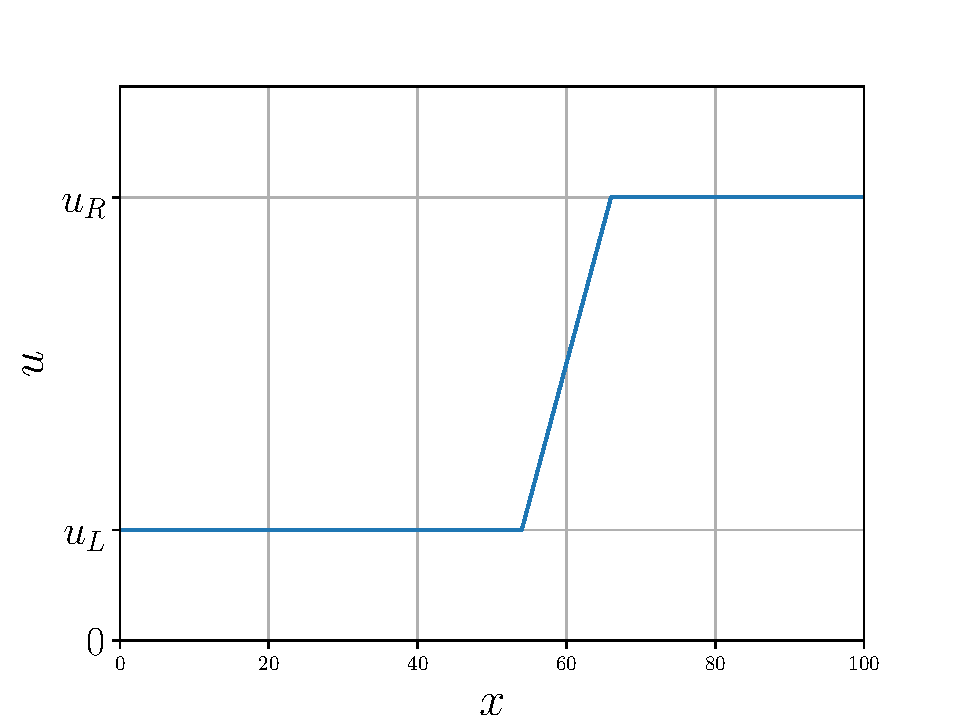
\includegraphics[width=\linewidth]{../some_plots/cap1/graficas/riemannRL-0.4.pdf}
	\end{subfigure}
	\begin{subfigure}{0.5\textwidth}
		\centering
		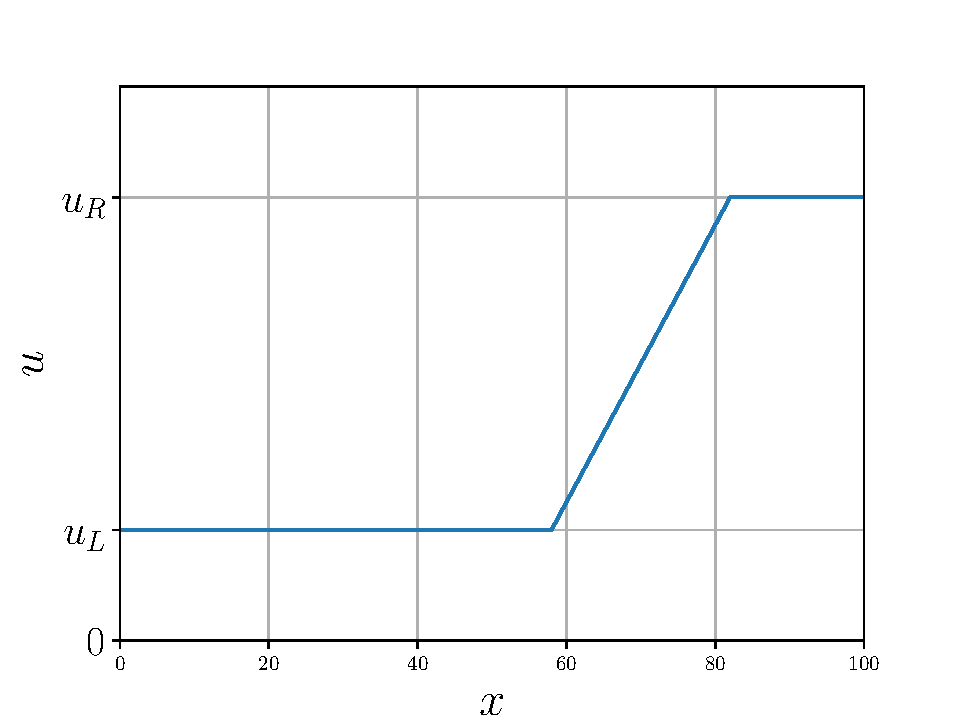
\includegraphics[width=\linewidth]{../some_plots/cap1/graficas/riemannRL-0.8.pdf}
	\end{subfigure}
	\begin{subfigure}{0.5\textwidth}
		\centering
		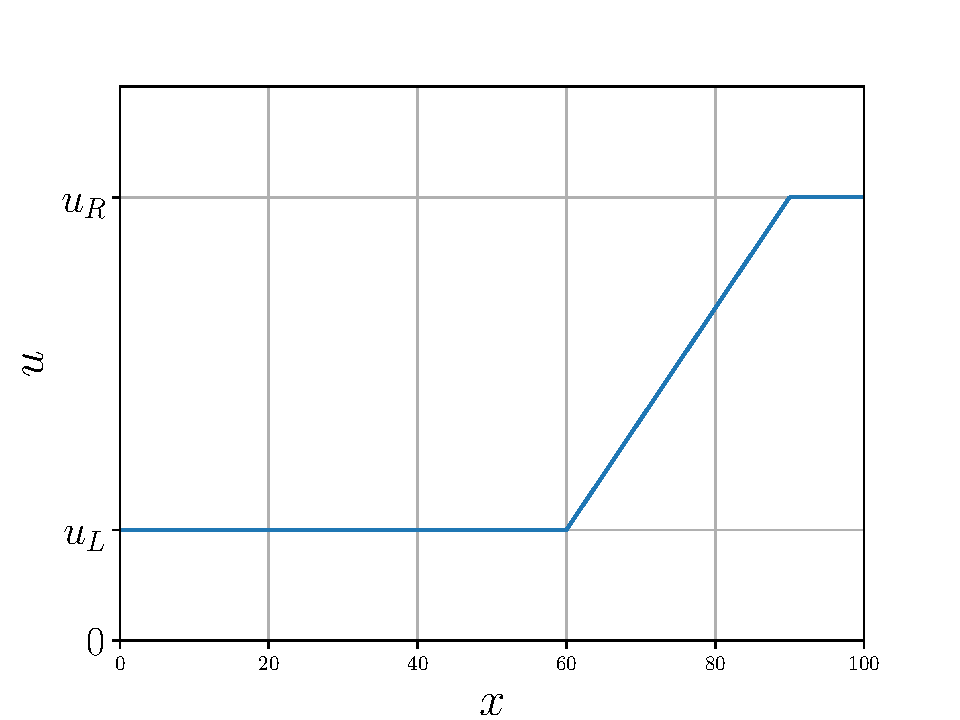
\includegraphics[width=\linewidth]{../some_plots/cap1/graficas/riemannRL-1.pdf}
	\end{subfigure}
	\caption{Gráficas de las soluciones, en distintos instantes de tiempo, de la ecuación de Burgers para el caso $u_L < u_R$ del problema de Riemann \textbf{Fuente:} elaboración propia.}
	\label{fig:rarefaccion}
\end{figure}
\section{Condiciones de entropía}
Se ha mencionado que la solución con viscosidad disipada es la solución débil correcta que debe considerarse al resolver una ecuación de conservación, sin embargo, resulta ser complicado encontrar la solución para una ecuación de conservación con viscosidad. Por lo tanto, se suelen imponer un conjunto de condiciones que sean equivalentes a aplicar el formalismo de viscosidad disipada. Estas se denominan \textbf{condiciones de entropía}, dado que cumplen un papel similar al de la entropía misma en problemas de la dinámica de los gases.

Existen varias versiones de la condición de entropía para una ecuación de conservación. Se mostraran las dos más relevantes con respecto a los métodos numéricos a tratar en este texto.
\subsection{Condición de entropía, primera versión}
La primera versión de la condición de entropía establece que una discontinuidad que se propaga a velocidad $s$ debe cumplir con la siguiente desigualdad
\begin{equation}
	f'(u_L) > s > f'(u_R)
	\label{eq:entropy}
\end{equation}
para que se satisfaga la misma condición. Para interpretar esta condición se debe resaltar que la derivada $f'(u)$ corresponde a la velocidad característica de la onda en un punto $(x,t)$. Por lo tanto, se puede notar que las curvas características se intersectan con la velocidad de propagación de la discontinuidad, de tal manera que las características a la izquierda de la onda de choque avanzan hacia el mismo choque y las características a la derecha son alcanzadas por la onda de choque.

Por otro lado, si se tuviese una discontinuidad que se propaga con una velocidad $s$ tal que se cumple la condición contraria, i.e., $f'(u_L) < s < f'(u_R)$, esta solución no sería estable ante alguna perturbación, ya sea al añadir una pequeña viscosidad o suavizando la discontinuidad en la solución. Al aplicar dichas perturbaciones, se generarían ondas de rarefacción en lugar de ondas de choque.

\subsection{Condición de entropía, segunda versión}
Esta condición desarrollada por Oleinik indica que si $u(x,t)$ es una solución débil físicamente válida si existe una constante $E >0$  tal que para todo $a>0$, $t>0$, sobre cualquier punto $x$ del dominio espacial se cumple que:
\begin{equation}
	\frac{u(x+a,t) - u(x,t)}{a} < \frac{E}{t}
\end{equation}.

\section{Sistemas hiperbólicos lineales}
El objetivo de esta sección es explicar la solución general de un sistema hiperbólico lineal y la solución del problema de Riemann asociado. Estos resultados serán de alta utilidad para construir la solución numérica que se busca en este texto.

El sistema descrito en la ecuación (\ref{eq:conserv-deriv-short}) con una función de flujo dada por $\mathbf{F}(\mathbf{U}) = \mathbf{A}\mathbf{U}$, siendo $\mathbf{A}$ una matriz con entradas constantes, es un sistema lineal de conservación. El sistema se puede escribir como
\begin{equation}
	\mathbf{U}_t + \mathbf{A}\mathbf{U}_x = 0
	\label{eq:linear-sys}
\end{equation}
donde $\mathbf{A} \in \mathbb{R}^{m \times m}$ y $\mathbf{U} : \mathbb{R} \times \mathbb{R} \rightarrow \mathbb{R}^{m}$. Formalmente hablando, este es un sistema lineal de $m$ cantidades conservadas. Naturalmente, también se define una condición inicial para este sistema,
\begin{equation}
	\mathbf{U}(x,0) = \mathbf{U}_{0}(x).
	\label{eq:cond-inicial-linear-sys}
\end{equation}

En la sección \ref{sec:ecuaciones-de-conservacion} se definió un sistema hiperbólico de primer orden como un sistema de la forma (\ref{eq:conservacion-jacobiana}) en donde los autovalores de $\mathbf{A}$ son todos distintos y son reales. De tal manera que si el sistema (\ref{eq:linear-sys}) es hiperbólico, se puede diagonalizar $\mathbf{A}$, i.e.,
\begin{equation}
	\mathit{\mathbf{A}} = \mathbf{R}\mathbf{\Lambda} \mathbf{R}^{-1}.
	\label{eq:a-diago}
\end{equation}
En esta relación, $\mathbf{\Lambda}$ es la matriz definida como $\text{diag}(\lambda_1, \lambda_2, \dots \lambda_m)$ donde $\lambda_i$ es el i-ésimo autovalor de $\mathbf{A}$. Mientras que $\mathbf{R}$ es la matriz formada por los autovectores columna de $\mathbf{A}$, denominados $\mathbf{r}_i$. Por ello, se tiene que
\begin{equation}
	\mathbf{A}\mathbf{r}_{p}  = \lambda_{p} \mathbf{r}_{p} 
\end{equation}
para todo $p \in [1,2,\dots, m]$.

\subsection{Resolución de un sistema hiperbólico lineal}
Se asumirá que se tiene un sistema de la forma (\ref{eq:linear-sys}), tal que los autovalores de $\mathbf{A}$ son todos distintos y reales, i.e., se trata de un sistema \textbf{estrictamente hiperbólico}. Este sistema se puede resolver introduciendo nuevas variables conocidas como \textbf{variables características}. Se define $\mathbf{v}$ como
\begin{equation}
	\mathbf{v} \equiv \mathbf{R}^{-1} \mathbf{U}.
	\label{eq:def-v}
\end{equation}
Por otro lado, se multiplica la ecuación (\ref{eq:linear-sys}) por $\mathbf{R}$
\begin{equation}
	\mathbf{R}^{-1}\mathbf{U}_t + \mathbf{R}^{-1} \mathbf{A} \mathbf{U}_x = 0,
\end{equation}
sustituyendo la expresión (\ref{eq:a-diago}) obteniendo,
\begin{equation}
	\mathbf{R}^{-1}\mathbf{U}_t + \mathbf{\Lambda} \mathbf{R}^{-1} \mathbf{U}_x = 0
\end{equation}
al usar el hecho de que $\mathbf{R}^{-1} \mathbf{R} = \mathbf{I}$. Luego, usando la definición de $\mathbf{v}$ (\ref{eq:def-v}) y dado que este ejemplo corresponde a un sistema lineal, las matrices $\mathbf{R}$ y su inversa son constantes, por tanto se tiene que
\begin{equation}
	\mathbf{v}_t + \mathbf{\Lambda} \mathbf{v}_x = 0
	\label{eq:diag-linear-sys}
\end{equation}.
Cabe destacar la similitud entre esta última ecuación y la ecuación (\ref{eq:linear-sys}). Sin embargo, la principal diferencia entre éstas es que la matriz $\mathbf{\Lambda}$ es una matriz diagonal y la matriz $\mathbf{A}$, en general, no lo es. Por tanto, el sistema definido en (\ref{eq:diag-linear-sys}) se puede desacoplar, obteniendo $m$ ecuaciones escalares lineales independientes. Esto es,
\begin{equation}
	(v_p)_t + \lambda_{p} (v_{p})_x = 0, \hspace{17mm} \forall p \in [1,2, \dots, m],
\end{equation}
donde $v_p$ es cada componente de $\mathbf{v}$. Este último sistema se resuelve usando el resultado de la ecuación de advección lineal escalar (\ref{eq:sol-advec}), obteniendo
\begin{equation}
	v_p(x,t) = v_p(x - \lambda_{p}t, 0)
	\label{eq:v-sub-p}
\end{equation}
dado que $v_p(x, 0)$ es la condición inicial para cada ecuación escalar según (\ref{eq:cond-inicial-linear-sys}).

Ya que se tiene la solución al sistema lineal en términos de las variables características, es oportuno escribir las soluciones en términos de las variables originales, i.e., $\mathbf{U}$. De forma que se tiene,
\begin{equation}
	\mathbf{v}(x,0) = \mathbf{R}^{-1} \mathbf{U}_0(x)
\end{equation}
y
\begin{equation}
	\mathbf{U}(x,t) = \mathbf{R} \mathbf{v}(x,t)
\end{equation}. Además $\mathbf{U}$ se puede escribir como una combinación lineal de los autovectores de $\mathbf{A}$, tomando en cuenta que el valor $\mathbf{v}_p$ es el coeficiente de cada autovector $\mathbf{r}_p$ en dicha expansión lineal, de tal manera que se tiene lo siguiente
\begin{equation}
	\mathbf{U}(x,t) = \sum_{p=1}^{m} v_p(x,t) \mathbf{r}_p
	\label{eq:sol-linear-sys}
\end{equation}
\begin{equation}
	\mathbf{U}(x,t) = \sum_{p=1}^{m} v_p(x - \lambda_p t, 0) \mathbf{r}_p
	\label{eq:sol-linear-sys-con-caracteristicas}
\end{equation}. Cabe destacar que, de forma similar al caso escalar, la solución $\mathbf{U}$ a este sistema lineal solo depende de la condición inicial $\mathbf{U}_0$ en los $m$ conjuntos de puntos, dados por $x - \lambda_p t$. Formalmente, su dominio de dependencia se escribe como $D(\bar{x}, \bar{t}) = \{x = \bar{x} - \lambda_{p} \bar{t}, \hspace{3mm} p = 1,2, \dots, m \}$.

De la misma manera que al generalizar el dominio de dependencia de una ecuación de advección lineal, se pueden introducir las curvas características asociadas a este sistema. El conjunto de características de la $p$ familia está dado por la ecuación $x'(t)=\lambda_{p}$. De tal manera que dichas curvas son de la forma $x = x_0 + \lambda_{p}t$ y se interpretan como rectas sobre el plano $x-t$, lo cual es consistente con el hecho de que se tratan de las características asociadas a un sistema lineal. El coeficiente $v_p(x,t)$ de cada autovector $\mathbf{r}_p$ es constante a lo largo de cada característica.

\subsection{Solución al problema de Riemann para un sistema hiperbólico lineal}
El problema de Riemann para un sistema hiperbólico lineal corresponde a la ecuación diferencial
\begin{equation}
	\mathbf{U}_t + \mathbf{A}\mathbf{U}_x = 0
\end{equation}
junto a la siguiente condición inicial
\begin{equation}
	\mathbf{U}_{0}(x) = 
	\begin{cases}
		\mathbf{U}_L, & x < 0 \\
		\mathbf{U}_R, & x > 0,
	\end{cases}
\end{equation}
considerando que este sistema es estrictamente hiperbólico.

Para resolver este problema, es conveniente escribir los dos estados $\mathbf{U}_L$ y  $\mathbf{U}_R$ en términos de los autovectores de $\mathbf{A}$, $\mathbf{r}_i$. Esta expansión se sustenta en la propiedad de independencia lineal que poseen los vectores $\mathbf{r}_i$ y dado que estos son $m$ distintos vectores,  indica que forman una base del espacio $\mathbb{R}^{m}$. Por tanto,
\begin{equation}
	\mathbf{U}_L = \sum_{p=1}^{m} \alpha_{p} \mathbf{r}_{p}
\end{equation}
\begin{equation}
	\mathbf{U}_R = \sum_{p=1}^{m} \beta_{p} \mathbf{r}_{p}
\end{equation}
con $\alpha_p$ y $\beta_{p}$ reales y constantes, para todo $p=1,2,\dots, m$.
Luego, utilizando la solución (\ref{eq:sol-linear-sys}) se obtiene
\begin{equation}
	v_p(x,0) = 
	\begin{cases}
		\alpha_p, & x < 0 \\
		\beta_{p}, & x > 0,
	\end{cases}
\end{equation}
y
\begin{equation}
	v_p(x,t) = 
	\begin{cases}
		\alpha_p, & \text{si} \hspace{4mm} x - \lambda_{p} t < 0 \\
		\beta_{p}, & \text{si} \hspace{4mm} x - \lambda_{p} t > 0,
	\end{cases}
\end{equation}
utilizando la relación del resultado (\ref{eq:v-sub-p}). Entonces, la solución al problema de Riemann tiene la forma (\ref{eq:sol-linear-sys-con-caracteristicas}), con $v_p$ definido como una función por partes.

Si se define a $P(x,t)$ como el valor máximo de $p$ tal que $x - \lambda_{p} t > 0$, entonces se puede escribir la solución al problema de Riemann como:
\begin{equation}
	\mathbf{U}(x,t) = \sum_{p=1}^{P(x,t)}\beta_{p}\mathbf{r}_{p} + \sum_{p=P(x,t) +1}^{m} \alpha_{p} \mathbf{r}_p
	\label{eq:sol-riemann-linear-sys-1}
\end{equation}.

Se puede verificar que esta solución cumple con la condición de salto de Rankine-Hugoniot (\ref{eq:rankinehugo}). Notando que al atravesar una curva característica $p$, el coeficiente de $\mathbf{r}_p$ salta de acuerdo a la siguiente expresión:
\begin{equation}
	\mathbf{U}_{Lp} - \mathbf{U}_{Rp} = (\beta_{p} - \alpha_{p})\mathbf{r}_p
\end{equation}
donde $\mathbf{U}_{Lp}$ y $\mathbf{U}_{Rp}$ son los valores de la onda a la izquierda y derecha de la curva característica $p$, respectivamente.

Tomando en cuenta que $\mathbf{F}(\mathbf{U}) = \mathbf{A}\mathbf{U}$, entonces:
\begin{equation}
 	\mathbf{F}(\mathbf{U}_{Lp}) - \mathbf{F}(\mathbf{U}_{Rp}) = \mathbf{A}(\mathbf{U}_{Lp} - \mathbf{U}_{Rp})
\end{equation}
\begin{equation}
	\mathbf{F}(\mathbf{U}_{Lp}) - \mathbf{F}(\mathbf{U}_{Rp}) = \mathbf{A}(\beta_{p} - \alpha_{p})\mathbf{r}_p
\end{equation}
\begin{equation}
	\mathbf{F}(\mathbf{U}_{Lp}) - \mathbf{F}(\mathbf{U}_{Rp}) = \lambda_{p}(\mathbf{U}_{Lp} - \mathbf{U}_{Rp}),
\end{equation}
con lo cual se demuestra que se cumple la condición Rankine - Hugoniot, notando que la velocidad de propagación de la discontinuidad es $\lambda_p$.

Otra forma útil de escribir la solución (\ref{eq:sol-riemann-linear-sys-1}) es a través de los saltos previamente desarrollados, esto es,
\begin{equation}
	\mathbf{U}(x,t) = \mathbf{U}_{L}(x,t) + \sum_{\lambda_{p} < x/t} (\beta_{p} - \alpha_{p}) \mathbf{r}_{p},
\end{equation}
o de forma equivalente,
\begin{equation}
	\mathbf{U}(x,t) = \mathbf{U}_{R}(x,t) - \sum_{\lambda_{p} \geq x/t} (\beta_{p} - \alpha_{p}) \mathbf{r}_{p}.
\end{equation}